\begin{tikzpicture}
\node[anchor=south west,inner sep=0] at (0,0) {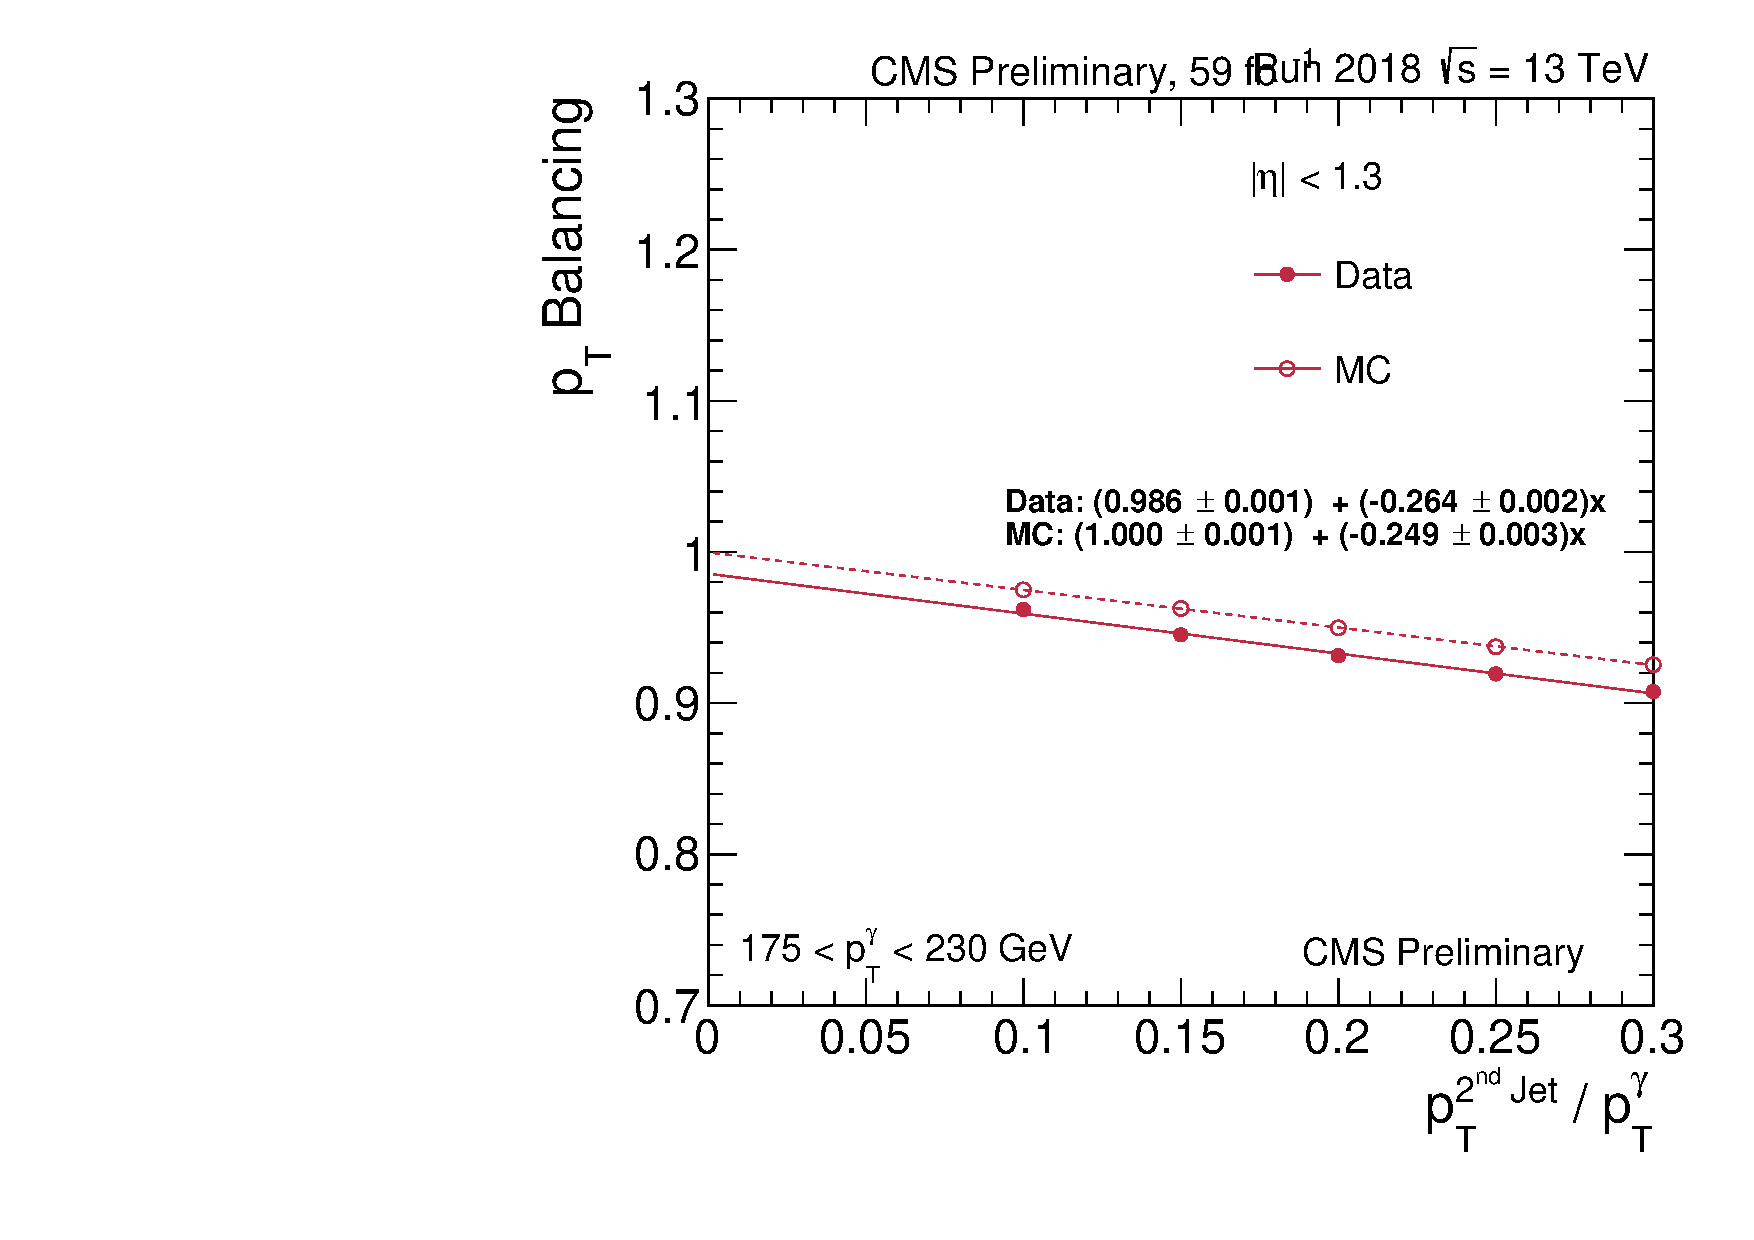
\includegraphics[width=8cm]{\PhDthesisdir/contents/chapter-JERC/plots/used/only_L2Res/Run2018ABCD/extrapolation/response_eta0013_ptPhot_175_230.pdf}};

% masks
\fill [white] (1.2, 7.31) rectangle (7.6,7.7);
\fill [white] (1, 0.15) rectangle (7.85,1.1);
\fill [white] (0, 1) rectangle (1.15,7.5);

% above txt
\draw (7.6, 7.5) node [left] {\footnotesize Run 2018 ABCD, \SI{59}{\femto\barn^{-1}} (\SI{13}{\TeV})};

% X axis
\foreach \val in {0, 0.05, 0.1, 0.15, 0.2, 0.25, 0.3}{
\draw ({1.2+(7.6-1.2)*\val/0.3}, .95) node {\small $\num{\val}$};
}
\draw (7, .5) node {$\alpha$};

% Y axis
\foreach \val in {0.7, 0.8, 0.9, 1, 1.1, 1.2, 1.3}{
\draw (1.25, {1.15+(7.25-1.15)*(\val-0.7)/(1.3-0.7)}) node [left] {\small $\num{\val}$};
}
\draw (.25, 7.25) node [left, rotate=90] {\Rbal};
\end{tikzpicture}
